\documentclass[conference]{IEEEtran}
\IEEEoverridecommandlockouts
% The preceding line is only needed to identify funding in the first footnote. If that is unneeded, please comment it out.
\usepackage{cite}
\usepackage{amsmath,amssymb,amsfonts}
\usepackage{algorithmic}
\usepackage{graphicx}
\usepackage{textcomp}
\usepackage{xcolor}
\usepackage[hyphens]{url}
\def\BibTeX{{\rm B\kern-.05em{\sc i\kern-.025em b}\kern-.08em
    T\kern-.1667em\lower.7ex\hbox{E}\kern-.125emX}}
\graphicspath{{figures/}}
% XeTeX (e.g. Tectonic) cannot use the Type 1 Times fonts IEEEtran selects
% under pdfLaTeX, and silently falls back to fonts without the bold and italic
% shapes the class needs. Load the TeX Gyre Times clones there only; pdfLaTeX
% (Overleaf, IEEE PDF eXpress) never enters this branch.
\usepackage{iftex}
\ifXeTeX
  \usepackage{fontspec}
  \setmainfont{texgyretermes}[Extension=.otf, UprightFont=*-regular,
    BoldFont=*-bold, ItalicFont=*-italic, BoldItalicFont=*-bolditalic]
  \setmonofont{texgyrecursor}[Extension=.otf, UprightFont=*-regular,
    BoldFont=*-bold, ItalicFont=*-italic, BoldItalicFont=*-bolditalic]
\fi
% Starts a new row of author blocks, so four long affiliations fit as 2x2
% instead of overflowing one row.
\makeatletter
\newcommand{\linebreakand}{%
  \end{@IEEEauthorhalign}
  \hfill\mbox{}\par
  \mbox{}\hfill\begin{@IEEEauthorhalign}
}
\makeatother
\begin{document}

\title{Ninsho: Design and Exploratory Evaluation of a Revocation-Oriented Session Management SDK for Node.js
\thanks{[FUNDING: state the funding agency, or delete this line if there is none.]}
}

% Student authors in the agreed order. Email/ORCID are placeholders until
% supplied. The project guide, Dr. Varsha Bhosale, is acknowledged below; add
% her as a fifth author block only if co-authorship has been explicitly agreed.
\author{\IEEEauthorblockN{Darshan Jain}
\IEEEauthorblockA{\textit{Department of Information Technology} \\
\textit{Vidyalankar Institute of Technology}\\
Wadala, Mumbai, India \\
{[email or ORCID]}}
\and
\IEEEauthorblockN{Yash Jadhav}
\IEEEauthorblockA{\textit{Department of Information Technology} \\
\textit{Vidyalankar Institute of Technology}\\
Wadala, Mumbai, India \\
{[email or ORCID]}}
\linebreakand
\IEEEauthorblockN{Chetna Padhi}
\IEEEauthorblockA{\textit{Department of Information Technology} \\
\textit{Vidyalankar Institute of Technology}\\
Wadala, Mumbai, India \\
{[email or ORCID]}}
\and
\IEEEauthorblockN{Chirag Sharma}
\IEEEauthorblockA{\textit{Department of Information Technology} \\
\textit{Vidyalankar Institute of Technology}\\
Wadala, Mumbai, India \\
{[email or ORCID]}}
}

\maketitle

\begin{abstract}
Node.js applications commonly assemble server-side sessions from separate token, cookie, rate-limiting and storage libraries, and the security of the result depends on how those pieces interact under concurrency and failure. This paper presents Ninsho, an open-source session management software development kit that makes revocation the organising constraint: opaque access tokens by default, single-use refresh tokens with family-wide reuse detection, optional PASETO version 4 public tokens with a deny-list, sender-constrained tokens through OAuth demonstration of proof of possession, and fail-closed behaviour when the shared store is unreachable. We describe the design and an evaluation built from recorded artifacts. The automated suite passed 2,150 tests against a real Redis instance at the evaluated commit, together with Docker-managed Redis persistence scenarios and browser regressions on three engines. An AI-assisted security assessment, using reproducible probe scripts, confirmed eight issues; the most serious allowed a revoked session's PASETO token to remain valid under a non-default clock tolerance and was fixed with a regression test. A single-machine benchmark compared configurations that provide the same server-side revocation guarantee. Median single-token verification took 1.59 ms for opaque tokens, 2.05 ms for PASETO and 2.16 ms for a JSON Web Token with an equivalent Redis lookup, against a Redis round trip of 1.34 to 1.59 ms, so the store lookup dominated verification cost here. With three trials and trial-to-trial throughput variation of up to about 30 percent among the compared configurations, the performance results are exploratory and do not establish a general advantage over JSON Web Token implementations.
\end{abstract}

\begin{IEEEkeywords}
authentication, session management, token revocation, refresh token rotation, DPoP, PASETO, Node.js, security evaluation
\end{IEEEkeywords}

% ═══════════════════════════════════════════════════════════════════════════
\section{Introduction}
\label{sec:intro}

A server that issues credentials must also be able to withdraw them. For a single Node.js service, the usual building blocks are a JSON Web Token (JWT) library~\cite{rfc7519}, a cookie handler, a rate limiter and a Redis client, combined in application code. Each component can be individually correct while the combination is not: a stateless token cannot be revoked before it expires unless the verifier consults shared state~\cite{rfc8725,rfc7009}; a rotated refresh token that is replayed carries the strongest available signal of theft, which is lost unless the whole token family is ended~\cite{rfc9700}; and a bearer token copied from a log or a compromised device is usable by anyone~\cite{rfc6750}. Measurement studies continue to find exploitable defects in JWT libraries themselves~\cite{yang2026jwt}, and session integrity in browsers remains an active research area~\cite{calzavara2017surviving,squarcina2023cookie}.

Ninsho~\cite{ninshorepo} is a monorepository of four TypeScript packages (\texttt{core}, \texttt{server}, \texttt{client}, \texttt{webauthn}) that packages these concerns behind one configuration object and deliberately excludes credential verification, which remains the application's responsibility. Its contribution is not a new primitive---all cryptography comes from \texttt{node:crypto} and WebCrypto---but a set of composition decisions that are hard to get right in application code, made the default, and tied to tests. The project's development rule is that a stated security property must name the test that demonstrates it.

This paper asks three research questions:
\begin{itemize}
\item \textbf{RQ1.} Which session-security properties does Ninsho enforce by default, and what executable evidence supports them?
\item \textbf{RQ2.} What does a probe-driven, AI-assisted security assessment find in a library that already carries a large passing test suite?
\item \textbf{RQ3.} What does server-side revocation cost per request in a measured environment, and how do opaque tokens, PASETO with a deny-list and a JWT with an equivalent deny-list compare when they offer the same revocation guarantee?
\end{itemize}

The contributions are: (i) a description of Ninsho's revocation-oriented design, including the ordering of store operations that makes refresh rotation, reuse detection and logout safe under concurrency (Section~\ref{sec:design}); (ii) an evaluation of its security behaviour combining 2,150 automated tests, Redis failure scenarios, browser regressions and an assessment whose findings are each reproduced by a probe script (Section~\ref{sec:security}); and (iii) a reproducible benchmark harness that separates verification cost from protected-request throughput and refuses to time any configuration that fails a security preflight (Section~\ref{sec:performance}). All quantitative results are tied to recorded artifacts and commits in an evidence map distributed with the manuscript.

% ═══════════════════════════════════════════════════════════════════════════
\section{Background and Related Work}
\label{sec:related}

\subsection{Self-contained and reference tokens}
A JWT carries signed claims and can be verified without contacting the issuer~\cite{rfc7519}. That property is also its revocation problem: a verifier that does not consult shared state accepts a token until its expiry regardless of logout. OAuth defines revocation~\cite{rfc7009} and introspection~\cite{rfc7662} endpoints, which reintroduce a server-side lookup. RFC 8725 records recurring JWT implementation pitfalls, including algorithm confusion~\cite{rfc8725}, and Yang et al.\ report vulnerabilities across 43 JWT implementations, 20 of which received CVE identifiers~\cite{yang2026jwt}. PASETO version 4 fixes the signature algorithm to Ed25519~\cite{rfc8032} in the token's version string and authenticates header, payload, footer and an implicit assertion through pre-authentication encoding (PAE), removing the negotiable \texttt{alg} header~\cite{pasetov4}. An opaque token, by contrast, is a random reference whose meaning lives entirely on the server, so deleting the record is revocation.

\subsection{Refresh-token rotation and reuse detection}
For OAuth 2.0~\cite{rfc6749}, the security best current practice requires that a refresh token presented after it has been rotated invalidate the active refresh token, because one of the two parties holding it must be an attacker and the server cannot tell which~\cite{rfc9700}. Implementing this correctly requires an atomic consume operation and a way to distinguish a legitimate parallel tab that lost a race from a replay minutes later. Fett et al.\ formally analysed OAuth 2.0 and identified attacks arising from the interaction of protocol steps~\cite{fett2016oauth}, which motivates treating ordering as part of the design rather than an implementation detail.

\subsection{Sender-constrained tokens}
OAuth Demonstrating Proof of Possession (DPoP) binds a token to a client-held key: each request carries a signed proof covering the HTTP method, target URI, a unique identifier and, when a token is presented, a hash of that token~\cite{rfc9449}. The token records the key's RFC 7638 thumbprint~\cite{rfc7638}. A stolen token is then useless without the key. DPoP does not defend against script running in the page, which can ask the browser to sign; it changes what an attacker who copies a credential can do afterwards.

\subsection{Web sessions and passkeys}
Surveys of web session security catalogue hijacking, fixation and integrity attacks and the defences against them~\cite{calzavara2017surviving}. Cookie hijacking at scale has been demonstrated against major services~\cite{sivakorn2016cookie}, and recent work shows that session integrity can be broken even with modern cookie protections~\cite{squarcina2023cookie}. Passwordless authentication through WebAuthn~\cite{webauthn3} replaces the secret the user remembers, but Lassak et al.\ document organisational obstacles to deploying it~\cite{lassak2024passkeys}, and Bonneau et al.\ show that no scheme dominates passwords on every usability, deployability and security criterion~\cite{bonneau2012quest}. Ninsho's optional WebAuthn package verifies ceremonies; it does not decide whether passkeys are appropriate.

\subsection{Gap addressed}
The standards above specify the individual mechanisms. Their composition in one service---which token format is the default, what happens when the store fails, how logout interacts with an in-flight rotation, where the DPoP binding is checked relative to a destructive consume---is left to implementers. This paper does not claim that Ninsho is the first library to combine these mechanisms; no systematic survey of Node.js session libraries was performed. It reports one composition, the decisions behind it, and evidence about how it behaves, including defects found in it.

% ═══════════════════════════════════════════════════════════════════════════
\section{System Design and Methodology}
\label{sec:design}

\subsection{Architecture and trust boundaries}
Fig.~\ref{fig:arch} shows the components. The \texttt{server} package exposes a single \texttt{Ninsho} facade that wires a token engine, a session manager, middleware, a rate limiter and one-time tokens to an injected store. Middleware is typed structurally against minimal request and response interfaces, so Express, Fastify, Hono and Koa are supported through adapters that import no framework. The application establishes identity itself and then calls \texttt{createSession()}. Route guards check roles, scopes, tenant and resource ownership; the ownership guard targets broken object-level authorization, the first entry of the OWASP API Security Top 10~\cite{owaspapi2023}, and refuses when the owner cannot be determined. Two boundaries carry the most risk: TB1, where attacker-controlled headers (\texttt{Authorization}, \texttt{DPoP}, \texttt{Host}, the request target) enter \texttt{verify()}; and TB4, where every security decision depends on a shared store whose availability and durability the library does not control.

\begin{figure}[htbp]
\centerline{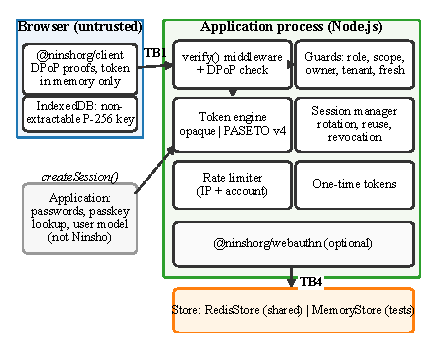
\includegraphics[width=\columnwidth]{fig-architecture.pdf}}
\caption{Ninsho components and the two trust boundaries discussed in the text. The application verifies credentials; Ninsho manages what follows. All session state crosses TB4 to the shared store.}
\label{fig:arch}
\end{figure}

\subsection{Defaults as security decisions}
Table~\ref{tab:defaults} lists the defaults of the evaluated release. The shortest configuration, \texttt{new Ninsho(\{store\})}, yields opaque tokens with no signing keys, five-minute access tokens and fail-closed store handling. Deviations---PASETO, fail-open, longer lifetimes---must be requested by name, and several emit a startup warning.

\begin{table}[htbp]
\caption{Security-relevant defaults (release 0.1.1)}
\begin{center}
\begin{tabular}{|l|l|}
\hline
\textbf{Setting} & \textbf{Default and rationale} \\
\hline
Token strategy & Opaque; deletion is revocation \\
Access token lifetime & 300 s \\
Refresh family lifetime & 604,800 s; never extended by rotation \\
Refresh grace window & 30 s for parallel tabs \\
Store failure mode & Closed: 503 rather than unchecked \\
DPoP proof age & 60 s; identifiers single-use \\
Clock tolerance & 5 s \\
\hline
\end{tabular}
\label{tab:defaults}
\end{center}
\end{table}

\subsection{Token lifecycle}
\emph{Issuance.} Opaque access and refresh tokens carry 256 bits from the operating system's random source and are stored only as SHA-256 hashes, so read access to the store yields no usable credential. The single exception is a short-lived grace mapping that holds the replacement refresh token for the grace window. PASETO access tokens carry \texttt{iss}, \texttt{aud}, time claims, the session identifier and, when bound, a \texttt{cnf} thumbprint inside the signed payload, so the binding cannot be stripped.

\emph{Verification.} Opaque verification hashes the token and reads one record; absence covers ``never existed'', ``expired'' and ``revoked'' alike, and clients receive one uninformative error. PASETO verification selects a key by the footer's key identifier, verifies the Ed25519 signature, validates claim shape and time, and then checks the token identifier against a deny-list. A store error raises a distinct error type so that the configured failure mode, not the verifier, decides whether the request proceeds.

\emph{Rotation and reuse.} Fig.~\ref{fig:refresh} summarises refresh handling in \texttt{session/manager.ts}. The DPoP binding is checked by reading the record \emph{before} the destructive consume; otherwise a thief holding the token but not the key could destroy the victim's session by presenting it. The consume itself uses the store's atomic \texttt{take} (Redis \texttt{GETDEL}), so exactly one of any number of concurrent callers rotates. The winner writes the replacement, then the grace mapping, then the tombstone that marks the old token as consumed; the order matters because a loser that sees a tombstone without a grace mapping revokes the family. Losers wait for the tombstone with bounded exponential backoff totalling about 126 ms, adopt the replacement inside the grace window, and otherwise revoke the family and emit \texttt{refresh.reuse\_detected}. Rotation carries the original authentication time forward, so a refreshed session never satisfies a step-up check.

\begin{figure}[htbp]
\centerline{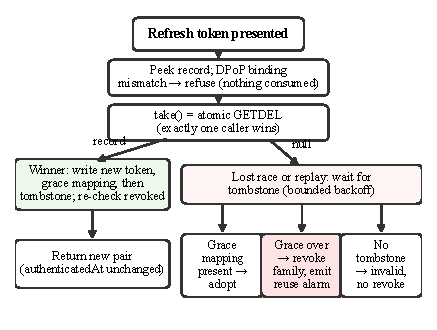
\includegraphics[width=\columnwidth]{fig-refresh-flow.pdf}}
\caption{Refresh handling. The binding check precedes the atomic consume; the winner publishes the grace mapping before the tombstone; the reuse response revokes the whole family.}
\label{fig:refresh}
\end{figure}

\emph{Revocation.} Revoking a session first writes a revoked marker, then enumerates and deletes the family's records and the engine's per-session token index. Creation, rotation and grace adoption re-check the marker after issuing an access token. Because the marker precedes every revocation read, either revocation finds the new token or the issuing path finds the marker; a regression test pins this interleaving for both strategies.

\subsection{Storage and failure modes}
The store contract has two operations that must be atomic: \texttt{take} for single-use credentials and \texttt{setIfAbsent} (Redis \texttt{SET NX EX}) for DPoP replay identifiers and one-time tokens. The Redis implementation disables the client's offline queue so that commands fail immediately during an outage rather than resolving after the HTTP request has timed out. Under \texttt{onStoreError: 'closed'}, an unreachable store produces 503. Under \texttt{'open'}, a PASETO token is admitted on its signature alone and an audit event records the admission; this disables revocation, DPoP replay protection and rate limiting for the duration of the outage. For opaque tokens the store holds the identity, so fail-open is rejected at configuration time.

\subsection{Evaluation methodology}
The evaluation used only the repository's code and artifacts recorded on 21 October 2026 on one machine (Table~\ref{tab:env}). It had three parts: the existing automated suites with a dedicated Redis instance; a security assessment in which every confirmed finding was reproduced by a probe script against the built packages before any fix; and a benchmark harness described in Section~\ref{sec:performance}. Source state matters because some fixes were made during the evaluation: the baseline tests ran on commit \texttt{6f82026} with a clean tree; the benchmark ran on the same commit plus the uncommitted F-01 fix, which changes only an index lifetime set at token issuance; and the final test run included all fixes. The published npm packages, version 0.1.1, were built from commit \texttt{f784566}, whose package sources differ from \texttt{6f82026} only in version strings; the published packages therefore contain the defects reported below, including those fixed during the evaluation. Each result is mapped to its source state in the accompanying evidence map.

\begin{table}[htbp]
\caption{Evaluation environment (recorded)}
\begin{center}
\begin{tabular}{|l|l|}
\hline
\textbf{Item} & \textbf{Value} \\
\hline
CPU & Intel Core i5-4300U, 2 cores, 4 threads \\
Memory & 16 GB; 2.3 GiB free at benchmark start \\
OS & Windows 10 Home 10.0.19045, Balanced plan \\
Runtime & Node.js 22.13.1, npm 11.0.0 \\
Store & Redis 7.4.11 in Docker Desktop (WSL2); \\
 & persistence disabled for the benchmark \\
Libraries & Express 5.2.1, ioredis 6.0.0, jose 5.10.0 \\
Co-running & Seven unrelated Kubernetes containers \\
\hline
\end{tabular}
\label{tab:env}
\end{center}
\end{table}

% ═══════════════════════════════════════════════════════════════════════════
\section{Security Evaluation}
\label{sec:security}

\subsection{Automated evidence}
With a dedicated Redis 7.4.11 instance, the full suite at commit \texttt{6f82026} passed 2,150 tests with none skipped: client 117, core 97, server 1,116, webauthn 623, the Express example 101, the interactive playground 95, and one HTTP demonstration test. Build and type checking passed. The suite includes a store contract run against both the in-memory and Redis stores, concurrency tests for rotation and revocation, PASETO tests against the specification's official vectors, and fuzz tests for parsers that receive attacker-controlled bytes, including the authenticator-data, DER and TPM parsers. After the fixes described below and their regression tests, the suite passed 2,152 tests. A consumer-scoped dependency audit of the four published packages reported no known vulnerabilities.

\subsection{Redis persistence, outage and data loss}
Seven Docker-managed scenarios start disposable Redis containers with controlled persistence; all seven executed and passed. A graceful restart with an RDB snapshot preserved sessions and revocation state for both strategies. During a temporary outage both strategies failed closed and recovered when Redis returned. After complete data loss, opaque sessions failed closed, because the record \emph{is} the token. PASETO tokens behaved differently: the deny-list was lost but signatures still verified, so \emph{previously revoked tokens became valid again until expiry}; restoring an older snapshot had the same effect for revocations made after it. The suite asserts this outcome rather than hiding it. Graceful shutdown was tested; abrupt process death, append-only-file durability and replica failover were not~\cite{redispersistence}.

\subsection{Browser lifecycle regressions}
Two Playwright scripts ran on Chromium 156, Firefox 157 and WebKit 27.2, and all six runs passed. The first opens two pages that initialise the IndexedDB key store concurrently and checks that both obtain the same non-extractable key, which survives reload. The second checks that a logout in one tab invalidates a peer tab through the opt-in broadcast channel and that a delayed refresh or sign-in response cannot restore an identity after logout. Cross-tab notices are best-effort and unauthenticated by design; suspended tabs, real cookie ordering and physical devices were not tested.

\subsection{Demonstration scenarios}
SecureShop, a demonstration application that installs the published packages, contrasts a deliberately limited stateless JWT baseline with Ninsho configurations. Fig.~\ref{fig:jwtreplay} shows the baseline accepting a copied token after client logout (HTTP 200). Fig.~\ref{fig:dpop} shows the DPoP configuration refusing a token presented without a proof, with a proof from another key, and with a replayed proof (HTTP 401 in each case). The baseline is a teaching device, not a representative JWT deployment: a JWT system can add a deny-list, as the benchmark's \texttt{jwt-redis} configuration does.

\begin{figure}[htbp]
\centerline{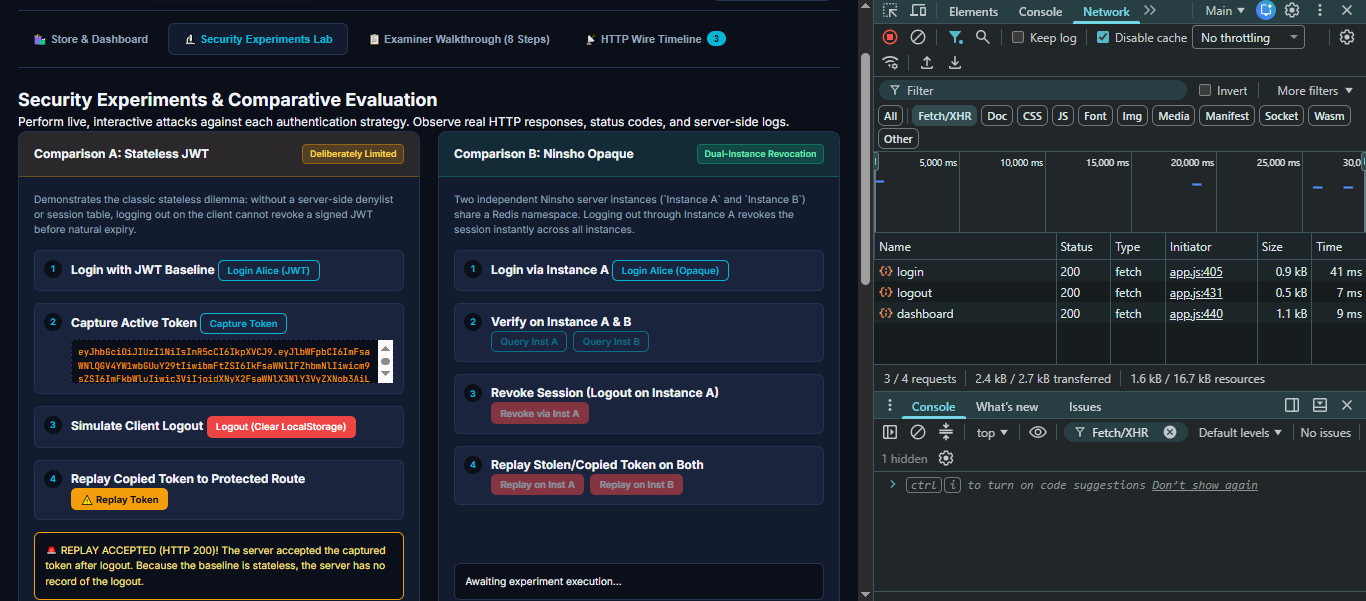
\includegraphics[width=\columnwidth]{fig-secureshop-jwt-replay.png}}
\caption{SecureShop, stateless JWT baseline: a token captured before client logout is replayed and accepted (HTTP 200); the network panel shows login, logout and the replayed request.}
\label{fig:jwtreplay}
\end{figure}

\begin{figure}[htbp]
\centerline{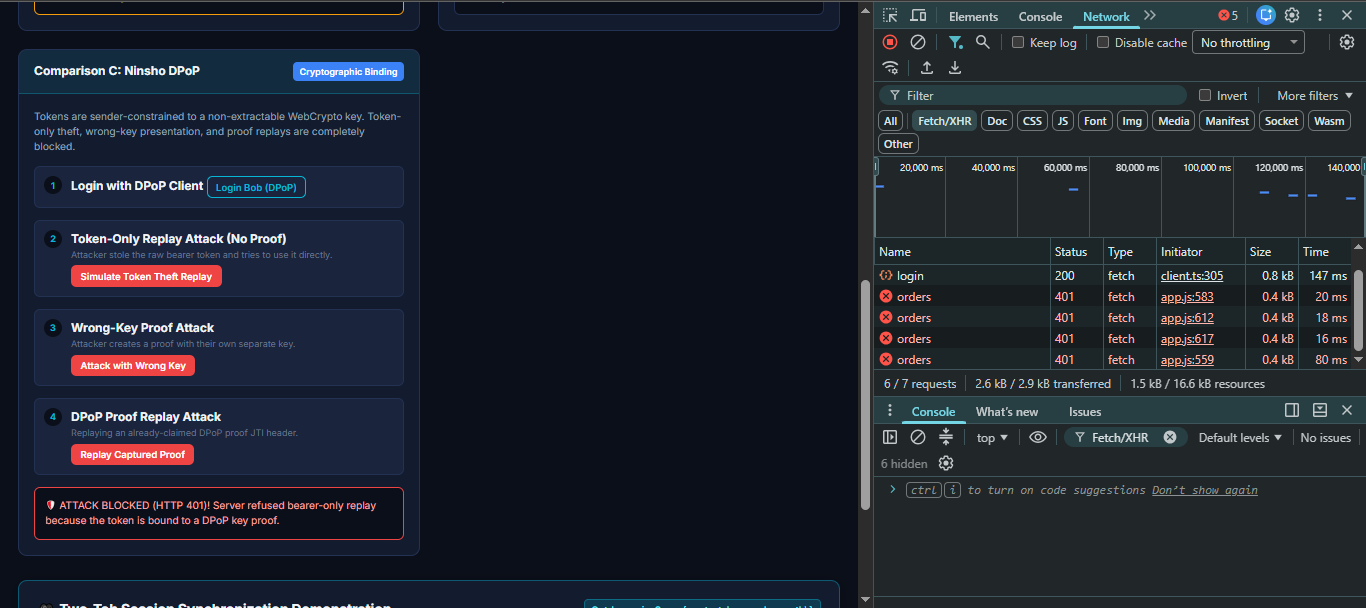
\includegraphics[width=\columnwidth]{fig-secureshop-dpop-attacks.png}}
\caption{SecureShop, Ninsho with DPoP: token-only, wrong-key and replayed-proof requests are each rejected with HTTP 401.}
\label{fig:dpop}
\end{figure}

\subsection{AI-assisted assessment}
The assessment was carried out by an AI coding assistant working in the project's repository with its test suites, and is \emph{not} an independent third-party audit. It read the session manager, both token engines, the Redis store, the HTTP and DPoP middleware, the rate limiter, one-time tokens, the browser client and the WebAuthn ceremony code in full, and other modules in part. For each suspected issue it wrote a probe against the built package and recorded the output; only reproduced issues were classified as confirmed. Table~\ref{tab:findings} lists them.

\begin{table}[htbp]
\caption{Confirmed findings of the assessment}
\begin{center}
\begin{tabular}{|p{0.7cm}|p{4.0cm}|p{1.2cm}|p{0.95cm}|}
\hline
\textbf{ID} & \textbf{Finding} & \textbf{Severity} & \textbf{Status} \\
\hline
F-01 & PASETO: revoked session's token keeps verifying when clock tolerance exceeds 60 s & High impact, low likelihood & Fixed, regression \\
F-02 & \texttt{trustProxy: false} honours forwarded addresses via framework \texttt{req.ip} & Medium & Open \\
F-03 & Logout racing rotation leaves a tombstone; stale tab raises a false reuse alarm & Low--Medium & Open \\
F-04 & One DPoP key yields several thumbprints (non-canonical base64url) & Low & Open \\
F-05 & CI guard cannot detect a skipped persistence suite & Low & Open \\
F-06 & Example app inherits a \texttt{proxy-addr} advisory & Info & Open \\
F-07 & Client rejects same-origin paths containing ``//'' & Low & Open \\
F-08 & Persistence tests can fail on container-name reuse & Low & Open \\
\hline
\end{tabular}
\label{tab:findings}
\end{center}
\end{table}

\emph{F-01.} Verification accepts a PASETO token until its expiry plus the clock tolerance, but the per-session index that revocation enumerates was kept for the access lifetime plus 60 s. Configuration permits a tolerance up to the access lifetime. With a tolerance above 60 s, an idle session's index expired first, so revoking the session wrote no deny-list entry and its token kept verifying for up to the tolerance minus 60 s. A probe through the public facade against real Redis, with both values set to 70 s, showed the token accepted after revocation at 134 s while a control session was refused; a regression test with fake time failed before the fix and passed after it, and the same probe then reported the token as revoked. The fix extends the index lifetime by the tolerance, matching the bound already used for deny-list entries. The default tolerance of 5 s is unaffected, opaque tokens are unaffected because their records expire at the token's expiry, and the fix is not part of the published 0.1.1 release.

\emph{F-02} was demonstrated over HTTP: with Express proxy trust enabled and Ninsho configured not to trust proxies, ten requests with rotating \texttt{X-Forwarded-For} values all succeeded against a per-address limit of three; with Express proxy trust disabled, the fourth was refused. The per-account bucket is unaffected. \emph{F-03} was reproduced on all four combinations of in-memory or Redis store and opaque or PASETO strategy: no credential is issued, but an application acting on the reuse alarm would act on a false positive. \emph{F-04} does not bypass binding, because a token is bound to one thumbprint, but a thumbprint cannot serve as a unique device identifier.

A second assessment pass found two further defects, each reproduced by a failing regression test and fixed: WebAuthn sign-in could return a user taken from the challenge or from the unsigned user handle when an integration omitted the stored credential's owner, and the demonstration's DPoP logout route passed the refresh cookie where a session identifier was expected, so the server session was not revoked. Potential concerns that were not demonstrated as defects include per-/128 bucketing of IPv6 addresses, the absence of path-length and key-usage checks on attestation intermediates, the absence of DPoP server nonces~\cite{rfc9449}, and the documented grace-window trade-off, in which a thief holding an unbound refresh token can obtain a fresh access token within 30 s of a legitimate rotation without raising an alarm.

% ═══════════════════════════════════════════════════════════════════════════
\section{Performance Evaluation}
\label{sec:performance}

\subsection{Harness and configurations}
The harness in \texttt{research/validation/benchmarks} answers two separate questions. Verification cost times one verification at a time in-process, and measures Redis round trips on their own so that the store component can be read off. Protected-request throughput runs each configuration as a separate server process behind the same Express 5 route returning the same 1,271-byte JSON body, driven by a closed-loop load generator with $N$ workers each holding one request in flight over a keep-alive connection.

Three configurations provide the same guarantee: a revoked credential is refused on the next request. \texttt{ninsho-opaque} performs a SHA-256 hash and one Redis \texttt{GET}. \texttt{ninsho-paseto} verifies an Ed25519 PASETO token and performs one Redis \texttt{EXISTS} on the deny-list. \texttt{jwt-redis} verifies an EdDSA JWT with the \texttt{jose} library~\cite{jose}, checks issuer, audience and time claims, and performs one Redis \texttt{EXISTS} through the same client library with the same failure posture (503 on store error). Using Ed25519 for both signed formats avoids comparing different signature algorithms by accident. Two references are reported but not compared: \texttt{jwt-stateless}, which omits the deny-list and therefore accepts revoked tokens until expiry, and \texttt{no-auth}, the floor for this application and machine. DPoP was excluded because a fair comparison would place a signing operation in the load generator on the same two cores and the JWT baseline has no equivalent.

Before timing, every configuration in every trial was sent a valid, missing, tampered, revoked and wrong-audience token; a comparable configuration that failed to refuse any of these would have aborted the run. All 15 preflights passed, and \texttt{jwt-stateless} accepted the revoked token, as expected.

The reported run used the harness's standard mode: three trials, each with 200 warm-up and 1,000 measured verifications per operation, and, for HTTP, 2 s of warm-up and 5 s of measurement at one and 16 concurrent clients. A five-trial mode was started but stopped to shorten the session; an earlier run aborted when tokens minted at start-up outlived their 300 s lifetime, a harness defect that was corrected before the reported run. Neither contributes any figure.

\subsection{Verification cost}
Table~\ref{tab:verify} and Fig.~\ref{fig:latency} report the median across trials of each trial's median (p50) latency, with the range across trials. The three revocation-checking verifiers took 1.59, 2.05 and 2.16 ms, against store round trips whose medians ranged from 1.34 to 1.59 ms. Verifying a signature without any store access took about 0.32 ms for both PASETO and JWT. Read together, these figures attribute most of each verification to the store round trip in this environment, with the signature adding a fraction of a millisecond for the signed formats. Tails were long: some trials recorded 99th-percentile store latencies above 15 ms.

\begin{table}[htbp]
\caption{Verification cost, concurrency 1 (ms)}
\begin{center}
\begin{tabular}{|l|c|c|c|}
\hline
\textbf{Operation} & \textbf{p50 median} & \textbf{p50 range} & \textbf{p95} \\
\hline
Redis \texttt{EXISTS} (ioredis) & 1.337 & 1.088--1.459 & 3.688 \\
Redis \texttt{GET} (Ninsho store) & 1.357 & 1.245--1.538 & 8.083 \\
Opaque + Redis & 1.588 & 1.200--1.743 & 7.679 \\
PASETO + deny-list & 2.051 & 2.043--2.217 & 5.938 \\
JWT + deny-list & 2.163 & 2.094--2.350 & 3.934 \\
\hline
PASETO, signature only$^{\mathrm{a}}$ & 0.323 & 0.241--0.491 & 0.801 \\
JWT, signature only$^{\mathrm{a}}$ & 0.320 & 0.301--0.513 & 0.603 \\
\hline
\multicolumn{4}{l}{$^{\mathrm{a}}$No server-side revocation; reference only. p95 is the median}\\
\multicolumn{4}{l}{\phantom{$^{\mathrm{a}}$}of the three trials' 95th percentiles.}
\end{tabular}
\label{tab:verify}
\end{center}
\end{table}

\begin{figure}[htbp]
\centerline{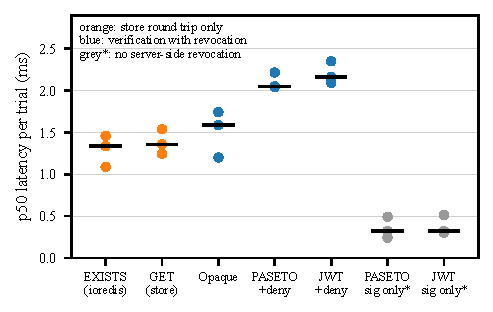
\includegraphics[width=\columnwidth]{fig-verify-latency.pdf}}
\caption{Per-trial p50 verification latency (dots, 1,000 samples per trial) and the median of the three trials (bars).}
\label{fig:latency}
\end{figure}

\subsection{Protected-request throughput}
Table~\ref{tab:http} and Fig.~\ref{fig:http} report throughput of successful responses; no non-200 response occurred during load. At one client the three comparable configurations had overlapping ranges (opaque 165--302, PASETO 226--275, JWT with Redis 213--261 requests/s), so no ordering is resolved. At 16 clients the opaque configuration reached a median of 951 requests/s with a narrow range (933--978), above JWT with Redis (801; 577--804) and PASETO (564; 420--567). The stateless JWT reference was roughly twice as fast as the comparable configurations at one client, which is the cost of the revocation lookup it omits, not an advantage of equal standing.

\begin{table}[htbp]
\caption{Protected-request throughput (successful req/s)}
\begin{center}
\begin{tabular}{|l|c|c|c|c|}
\hline
 & \multicolumn{2}{c|}{\textbf{1 client}} & \multicolumn{2}{c|}{\textbf{16 clients}} \\
\cline{2-5}
\textbf{Configuration} & \textbf{Median} & \textbf{CV} & \textbf{Median} & \textbf{CV} \\
\hline
Ninsho opaque & 287 & 29.8\% & 951 & 2.4\% \\
Ninsho PASETO & 245 & 9.9\% & 564 & 16.2\% \\
JWT + Redis deny-list & 251 & 10.4\% & 801 & 17.9\% \\
\hline
JWT stateless$^{\mathrm{a}}$ & 488 & 10.0\% & 963 & 34.1\% \\
No authentication$^{\mathrm{a}}$ & 1,136 & 5.0\% & 1,310 & 5.4\% \\
\hline
\multicolumn{5}{l}{$^{\mathrm{a}}$Reference only; not an equivalent guarantee. CV: coefficient}\\
\multicolumn{5}{l}{\phantom{$^{\mathrm{a}}$}of variation of throughput across three trials.}
\end{tabular}
\label{tab:http}
\end{center}
\end{table}

\begin{figure}[htbp]
\centerline{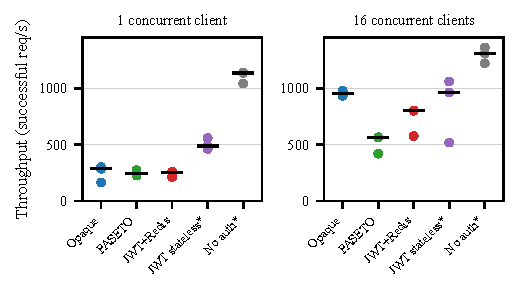
\includegraphics[width=\columnwidth]{fig-http-throughput.pdf}}
\caption{Per-trial throughput (dots, 5 s each) and medians (bars). Starred configurations are references without an equivalent revocation guarantee.}
\label{fig:http}
\end{figure}

% ═══════════════════════════════════════════════════════════════════════════
\section{Results and Discussion}
\label{sec:discussion}

\emph{RQ1.} The defaults in Table~\ref{tab:defaults} are each backed by named tests, and the evaluation reproduced them: rotation with family-wide reuse response, revocation that survives concurrent issuance, fail-closed behaviour during an outage, and DPoP rejection of token-only, wrong-key and replayed-proof requests. The evidence also shows where the guarantees end. The PASETO strategy's deny-list is only as durable as Redis; after data loss, revoked tokens revive, while opaque sessions fail closed. Choosing PASETO buys verification without a store at the price of revocation that depends on store durability, and choosing fail-open buys availability at the price of every store-backed control.

\emph{RQ2.} A suite of more than two thousand passing tests did not prevent the assessment from confirming eight issues and, in a second pass, two more. F-01 is instructive: an earlier fix had already aligned the deny-list lifetime with the clock tolerance, and the sibling index was missed. Most findings sit at a boundary between Ninsho and something it does not own---a framework's proxy setting (F-02), the base64url encoding of a client-supplied key (F-04), the CI runner (F-05), a container runtime (F-08)---or in an interleaving that only a deliberately paused store exposes (F-03). Writing a probe for each suspicion before classifying it kept the classification honest: several suspicions were refuted on inspection, including a backup-flag check that the parser does enforce. The assessment remains model-assisted and selective; attestation formats, parsers and two framework adapters were covered mainly by their existing suites.

\emph{RQ3.} In this environment the revocation lookup dominated verification: each revocation-checking verifier exceeded the matching bare round trip by only about 0.2 to 0.8 ms, and dropping the lookup roughly halved single-client request latency (p50 3.74 to 1.89 ms) and doubled throughput. Opaque tokens avoided the signature cost and showed the lowest median verification latency and the highest 16-client throughput. Two observations limit what can be said beyond that. First, PASETO and JWT with Redis perform the same primitive and the same single lookup, yet differed at 16 clients; no profiling was done, so the cause is unexplained. Second, the shuffled order happened to run PASETO fourth and JWT with Redis fifth in all three HTTP trials, so their comparison is confounded with position in the run, and the third trial, in which both dropped, is consistent with drift. The results describe one laptop, one JWT library and a Redis reached across a virtualisation boundary; they do not establish that opaque tokens or Ninsho are faster than JWT-based systems in general.

% ═══════════════════════════════════════════════════════════════════════════
\section{Threats to Validity and Limitations}
\label{sec:threats}

\emph{Internal validity.} Load generator, server and Redis shared two physical cores with seven unrelated containers. Each HTTP cell is three 5 s windows; three trials give a median and a range but no meaningful confidence interval, and throughput variation reached a coefficient of variation of 29.8\% among comparable cells and 34.1\% for the stateless reference. Configuration order was not balanced, as noted above. The harness is plain JavaScript outside the project's type checking; it guards against drift by using the public facade and by its security preflight.

\emph{Construct validity.} Loopback HTTP measures server cost plus the Node.js HTTP client, without network latency. Persistence was disabled to keep disk I/O out of the measurement. The JWT baseline is one carefully specified configuration; caching, introspection or a different library would change the numbers.

\emph{External validity.} Results come from Windows 10 and Node.js 22 only; the project's continuous integration covers Node.js 20 and 22 on Linux for the evaluated commit, but the fixes made during the evaluation were not run there. Browser results use automation builds and stubbed networking, not physical devices. No user study or production deployment was performed.

\emph{Assessment validity.} The security assessment was performed by an AI coding assistant and is not an independent audit. Passing tests and a clean probe do not demonstrate the absence of vulnerabilities. Seven of the eight confirmed findings remain open. The F-01 fix and the two later fixes exist in the working tree of the evaluated commit and are not in the published release.

% ═══════════════════════════════════════════════════════════════════════════
\section{Conclusion and Future Work}
\label{sec:conclusion}

Ninsho makes revocation the organising constraint of a Node.js session library: opaque tokens by default, refresh rotation whose ordering is designed for concurrency, sender-constrained tokens, and refusal rather than guesswork when the store cannot be reached. The evaluation supports these behaviours under the tested conditions, identifies where they depend on deployment choices---most clearly PASETO's reliance on a durable deny-list---and shows that a probe-driven assessment found real defects in code that already passed an extensive suite. On the measured machine, the store round trip, not the token format, accounted for most of the verification cost among configurations with equal revocation guarantees.

Future work should repeat the benchmark on Linux hosts with a local Redis, balanced configuration order, more and longer trials, and profiling of the signed-token paths; resolve the open findings, in particular F-02; add durability guidance and tests for append-only persistence and replica failover; offer IPv6 prefix aggregation and DPoP server nonces; evaluate integration effort with developers new to the library; and obtain an independent security review.

\section*{Acknowledgment}
The authors thank their project guide, Dr. Varsha Bhosale, Department of Information Technology, Vidyalankar Institute of Technology, Mumbai, for supervising this work. [Add any further acknowledgments agreed by all authors, or delete this sentence.]

\section*{Disclosure of AI Assistance}
[AUTHORS TO COMPLETE according to the target venue's and institution's policy.] Factual basis for the statement: the security assessment, the probe scripts, the benchmark harness and its figures, and a draft of this manuscript were produced with an AI coding assistant (Anthropic Claude) working in the project repository. [State which parts the authors wrote, reviewed and verified, and confirm that all authors accept responsibility for the content.]

\bibliographystyle{IEEEtran}
\bibliography{references}

\end{document}
